\chapter{Conclusion}
\label{chp:conclusion} 

\section{Future Work}

\subsection{Autonomous Non-Destructive Testing}

Advancements in \ac{AI}, big data and machine learning opens up exciting possibilities for autonomous \ac{NDT}. Branches of this technology is usually encountered in the context of image recognition, i.e. teaching machines to understand what they see. The same concepts may be applied to forms of \ac{NDT} besides regular visual sensor input, such as ultra sound or eddy currents for corrosion detection.  

\subsection{Large Scale Kinect Fusion - Kintinous}

Kinect Fusion has great potential for augmented reality. Augmented reality is a concept which blends the real and virtual environment. This opens up opportunities to create realistic and immersive training scenarios for the operators. Unfortunately, Kinect Fusion is limited reconstructing a rather small volume depending on the resolution. By varying the resolution, volumes can at the least cover a normal office desk and at the most cover a small room \cite{keylist}.  

Kintinous...

A guide on how to build Kintinous can be found  at \href{Github}{https://github.com/mp3guy/Kintinuous}. The procedure is complicated, as it usually is for experimental builds. It is recommended to attempt the procedure on a fresh install of Ubuntu 14.04 or 15.04 \cite{Kintinous}.

\subsubsection{Improve the Communication Protocols}

Communication between \ac{ROS} and the XMEGA A3BU, the Bluetooth device and the \ac{OCS}, all use the same pattern: A start byte \texttt{'':''}, the message with the speed setting and a stop byte \texttt{''Esc''}. In later projects, it could be beneficial to implement a more robust and rich communication protocol with more options for remote operation. 

\subsubsection{Implement a Fully Functional Operator Control Station}

At the end of this project, the \ac{OCS} provided functionality for moving the robot, and displaying live video from the Kinect. 

\subsection{Hardware}

Several hardware-related issues became apparent over the course of the project - especially toward the final weeks. These issues are likely the results of many disconnected projects on the same hardware.

\subsubsection{Kinect Sensor Location}

This is the first semester in which a Kinect has been used on the robot. At the moment, the sensor is placed directly over the \ac{LIDAR} device. Because the depth sensor in the Kinect for XBOX 360 has a minimum range of roughly $0.5 m$, it cannot detect objects within reach of the robot arm. It is recommended to find a new location further back on the robot. 

\subsubsection{Combine Stereo Cameras with Kinect-like Sensors}

As mentioned, both active and passive depth cameras have limitations. The Kinect does function in direct sunlight, but it can measure depth in the dark. Passive depth sensors, for example stereo cameras, does depend on visible light to sense anything at all. While RTAB-Map does depend on visibility for loop closure detection, there are  other \ac{SLAM} methods, e.g. \textit{Kinect Fusion}, which do not. An implementation could use a light sensor to sense light that may interfere with the Kinect. Light levels could be compared to a threshold and switch between the stereo cameras or the Kinect depending on how well each sensor will work in the current conditions. 

\subsubsection{On-board Computer Suitable for Moving Platforms}

Because this author used his own computer to control the robot, all features related to \ac{ROS} was removed from the robot at the end of the project. A new computer should be equipped with \ac{SSD} storage

\subsubsection{Wheels}

\begin{wrapfigure}{r}{0.5\textwidth}
	\vspace{-20pt}
	\begin{center}
		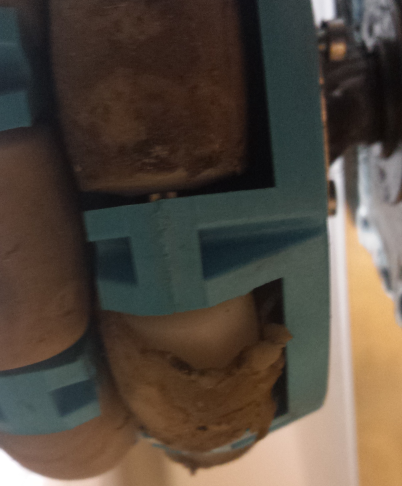
\includegraphics[width=0.48\textwidth]{worn_wheel2}
	\end{center}
	
	\caption{Worn omniwheel}
	\label{fig:worn_wheel}
	%\vspace{-20pt}
\end{wrapfigure}

There were mainly two issues with the omni-wheels this semester: They are worn out, and one wheel slipped out of the motor drive shaft. The rubber on a few of the perpendicular rollers is loose and about to fall off the plastic rims. This causes the robot to shake, which can damage spinning hard disk drives or shake the sensors out of their calibrated positions.   

A new set of wheels should be able to carry the weight of the robot, and enable the robot to drive over small barriers such as door sills and steel grates. This will most likely prompt a redesign of the mobile base.

\section{Final Conclusion}

A mobile robot platform has been fitted with a new software framework capable of \ac{SLAM} and autonomous navigation in two dimensions. The software framework, \ac{ROS}...

The \ac{SLAM} system is configured to use a Kinect for Xbox 360 in combination with a \ac{LIDAR} to generate 2D occupancy grid maps and 3D point cloud maps of the environments. The mapping system, \ac{RTAB-Map} use visual features to The current implementation is capable of building maps over multiple sessions. Scan matching from Hector SLAM provides odometry to \ac{RTAB-Map}. Using laser scans as a source of odometry was susceptible to errors in featureless areas, when the robot rounded corners and when people walked by the robot. 

The navigation stack in \ac{ROS} has been configured for this mobile base, and enables the robot to autonomously move towards a goal location in a 2D map. 

Navigation tests on the live robot showed that the robot can navigate successfully in known and structured environments with some room manoeuvring space. Navigation performance decreased in cluttered environments, e.g. office environments with many tables placed closely together.

The Kinect and the LIDAR is currently placed in the front of the base. As the Kinect is unable to reliably measure depth any closer than $0.8 m$.

Two supporting tools, an Android device and a remote \ac{OCS} was also developed.